\part{Fundamentação Teórica}
\chapter[Fundamentação Teórica]{Fundamentação Teórica}

\section{Inteligência artificial}
    \subsection{O que é?}
        A inteligência artificial pode ser definida sob diversos pontos de vista os quais podem dizer respeito tanto a capacidade de pensamento quanto a capacidade raciocínio dos agentes inteligentes quando comparados a seres humanos no caso de pensamentos, e a sistemas ideais no caso do raciocínio. \cite{norvig2014inteligencia}
Sendo assim, pode-se entender inteligência artificial como o ramo da computação onde se propoe criar dispositivos inteligentes capazes de simular uma atividade humana, sendo ela um pensameno, um raciocínio ou mesmo uma atitude.
    \subsection{Redes Neurais Artificiais}
        \subsubsection{Inspiração biológica}

    O cérebro humano possui um tipo específico de célula que aparentemente nao se regenera lentamente como as outras. A estas células são atribuidas nossa capacidade de pensamento, lembranças e transferência de todo tipo de informações para todo o corpo. Estas células chamadas neurônios estão presentes em cifras de 100 bilhões de unidades. \cite{anderson1992artificial}
    O neurônio é dividido em basicamente três partes: núcleo, axônio e dendritos, e cada uma delas tem sua atividade bem estipulada. O núcleo é onde ocorre todo o processamento dos sinais elétricos recebidos pelos dendritos que ficam nas extremidades da célula e são transmitidos pelo axônio para o próximo neurônio.

    \begin{figure}[ht]
        \centering
        \label{fig01}
            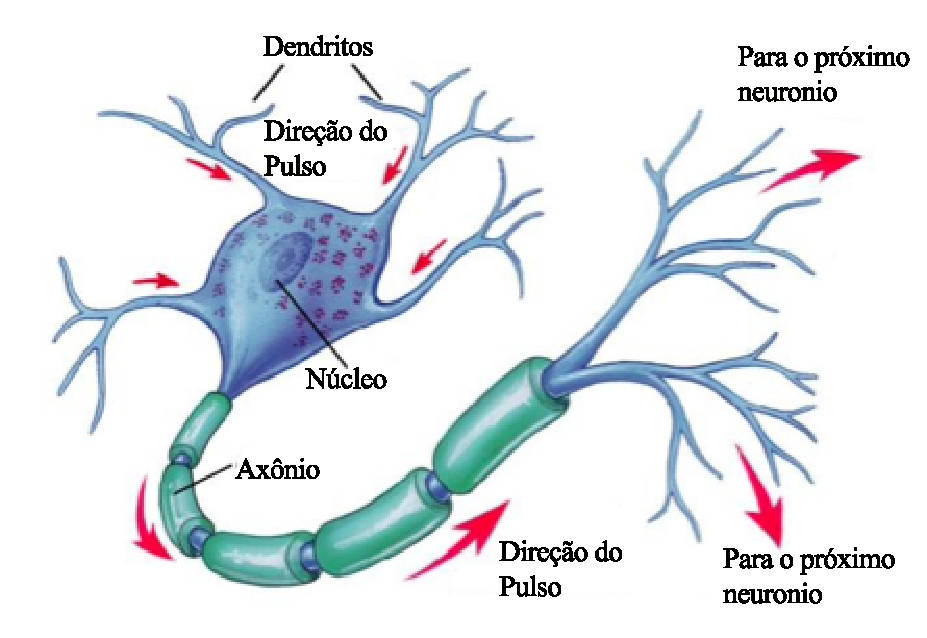
\includegraphics[keepaspectratio=true, scale=0.4]{editaveis/images/neuronio.eps}
        \caption{Representação de neurônio humano}
        Fonte: \url{http://goo.gl/vbd7T6}
    \end{figure}

    Estes pulsos, ou sinais elétricos, são transmitidos do axônio de um neurônio para os dendritos de um outro neurônio através das fendas sinapticas, ou sinápses.

    \begin{figure}[ht]
        \centering
        \label{fig02}
            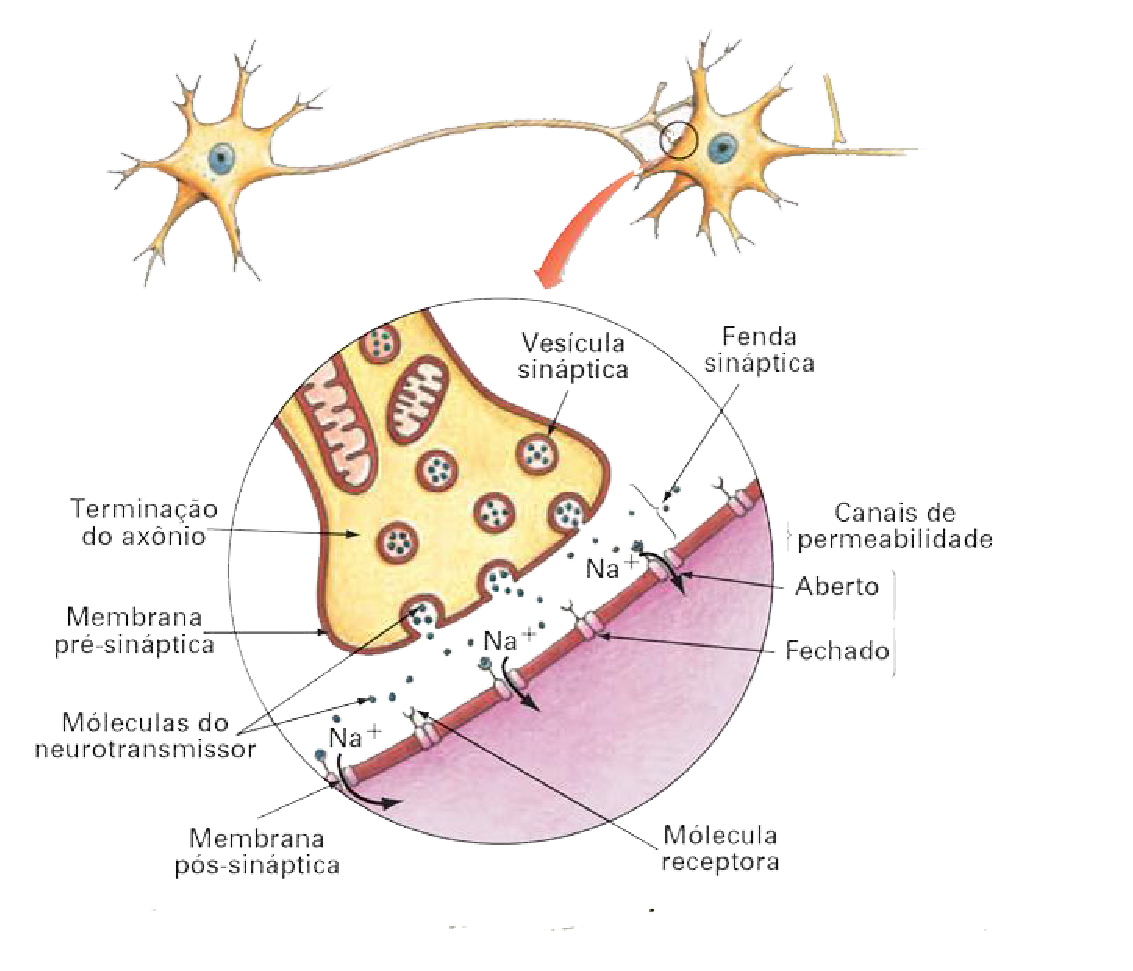
\includegraphics[keepaspectratio=true, scale=0.4]{editaveis/images/sinapse.eps}
        \caption{Representação de uma sinápse.}
        Fonte : \url{http://goo.gl/TCtvVG}
    \end{figure}

    As sinápses são regiões ativas eletroquimicamente entre as membranas celulares dos neurônios, onde a partir de uma excitação ocorre uma reação química que transmite os sinais de uma célula a outra por intermédio de substancias chamadas neurotransmissores.

\subsubsection{Modelagem matemática}
    O neurônio biológico pode ser modelado matematicamente de um modo que inspire a criação de um neurônio artificial a partir dessa divisão. Sendo assim, uma modelagem matemática de um neurônio biológico é: \cite{rocha2006}

    \begin{itemize}
        \item Entrada: São os dendritos, por onde os sinais chegam;
        \item Pesos: São as áreas onde as informações são transferidas de um neurônio para outro,  ou seja as sinápses;
        \item Soma: É o núcleo do neurônio, onde cada entrada é multiplicada com seu devido peso para que em seguida passe por uma função de transferência, a qual vai gerar os sinais de saída dos axônios;
        \item Função de Transferência: É o potencial necessário para ativação das fendas sinápticas.
        \item Saída: São os axônios do neurônio biológico.
    \end{itemize}

    Dessa maneira, tomando por base este modelo, o desenho de um neurônio artificial seria:

    \begin{figure}[ht]
        \centering
        \label{fig03}
            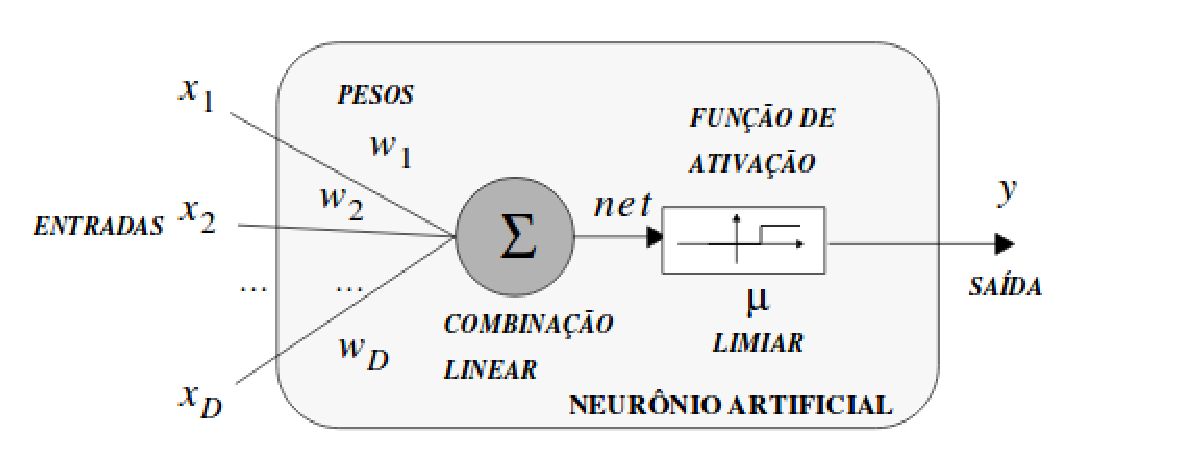
\includegraphics[keepaspectratio=true, scale=0.27]{editaveis/images/modeloNeuronio.eps}
        \caption{Representação matemática do neurônio.}
        Fonte : \url{http://goo.gl/iD2fg4}
    \end{figure}
    \newpage

\subsubsection{Perceptron de Multiplas Camadas}
    O \textit{perceptron} é a menor unidade de processamento, e representa um neurônio conforme a representação da figura 3(\ref{fig03}). Uma rede perceptron de multiplas camadas, ou MLP, é composta de camadas de perceptrons alinhados em diferentes camadas, que podem variar a partir de três. A primeira é a camada de entrada, por onde os dados entram na rede, a segunda é uma camada intermediária de processamento, normalmente chamada de camada escondida e a ultima é a camada dos neurônios de saída, que mostram a resposta. Um modelo básico de MLP é descrito na figura 4(\ref{fig04}) a seguir:

    \begin{figure}[ht]
        \centering
        \label{fig04}
            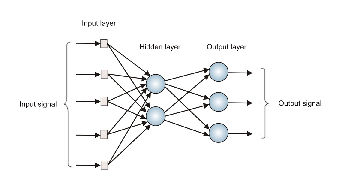
\includegraphics[keepaspectratio=true, scale=2.1]{editaveis/images/mlp.eps}
        \caption{Representação de uma MLP.}
        Fonte : \url{http://goo.gl/ICaZBQ}
    \end{figure}



    \subsection{Treinamento Backpropagation}
        \textit{Backpropagation} é um algorítmo de aprendizagem normalmente aplicado a MLP's que visa a aprendizagem baseada em correção de erros. Isso ocorre devido à retropropagação dos erros de saída de uma RNA pelas camadas anteriores, para que assim sejam balanceados os pesos de entrada da rede.
Este algorítmo possui três fases distintas:

\begin{itemize}
    \item Fase 1: Propagação dos sinais \\ Os sinais são propagados juntamente com os valores de entrada por todos os neurônios da rede a partir da entrada de dados até a camada de saída.
    \item Fase 2: Cálculo dos erros \\ Os erros são calculados nos neurônios de saída da rede para que sejam retropropagados.
    \item Fase 3: Retropropagação dos erros \\ Os erros que são encontrados nas camadas de saída, são propagados de volta para as camadas anteriores rebalanceando os pesos de entrada nas camadas superiores da rede. \cite{netto2006} Dessa forma a rede poderá chegar a resultados mais exatos nas próximas interações.
\end{itemize}

As duas fases descritas podem ser observadas na figura a seguir:

\begin{figure}[ht]
        \centering
        \label{fig05}
            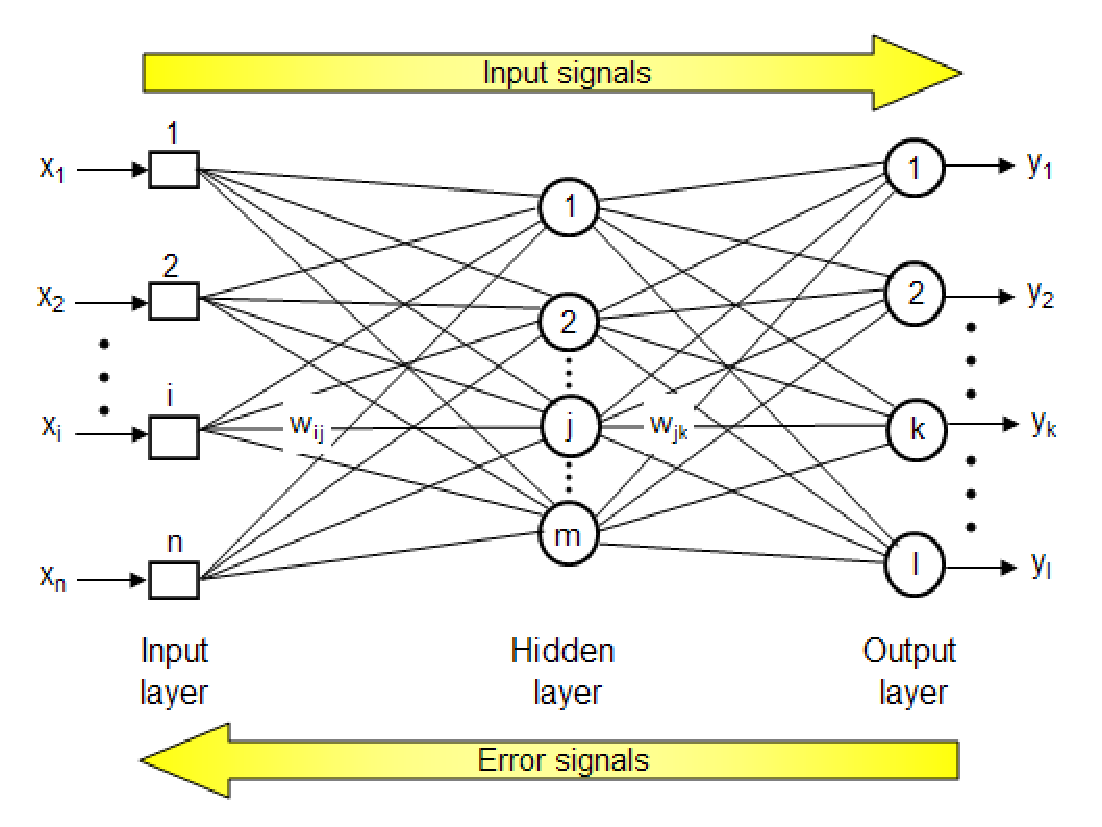
\includegraphics[keepaspectratio=true, scale=0.4]{editaveis/images/backprop.eps}
        \caption{Propagação de sinais de entrada e erros no \textit{Backpropagation}.}
        Fonte : \url{https://goo.gl/o7IGy4}
\end{figure}



\section{Aprendizado de Máquina}
    Aprendizado de máquina (ou \textit{Machine learning} - ML) é uma sub área da inteligência artificial voltada à otimizar critérios de desempenho de acordo com análise de dados e ocorrências passadas. \cite{alpaydin2010} Uma das características mais marcantes da ML é a análise de conjuntos de dados para automatizar o desenvolvimento de modelos analíticos para suas funcionalidades, isso quer dizer que de acordo com essas análises e com dados de ocorrências já conhecidas por uma aplicação baseada em ML, o aprendizado possibilita às aplicações reagirem de maneira autônoma à eventualidades para as quais não foram programadas.

Aprendizado de máquina normalmente é utilizado em duas situações que podem ser enxergadas pela análise do problema:

\begin{itemize}
    \item Complexidade elevada do problema: \\ Por exemplo, tarefas rotineiras que seres humanos executam, mas que para serem programadas o algorítmo teria uma complexitade enorme como dirigir ou reconhecer imagens. Outro exemplo é a necessidade de um processamento de uma massa de dados muito grande.
    \item Necessidade de adaptabilidade do sistema: \\ Por exemplo, detecção de diversos tipos de spam, para marcar mensagens. \\ \cite{shalev2014}
\end{itemize}

\subsection{Fluxo de trabalho}
    O fluxo de trabalho básico de ML consiste em duas fases, a de construção de um modelo e a de predição. Na primeira são utilizados dados históricos (ou dados de treinamento) para um ciclo de modelagem onde será definido, evoluido e otimizado um modelo de dados para que o algorítmo o consuma, realizando assim um tipo de aprendizado. É a partir deste modelo otmizado que o algorítmo vai conseguir fazer predições sobre novos dados ou ainda categorizações.

    \begin{figure}[ht]
            \centering
            \label{fig06}
                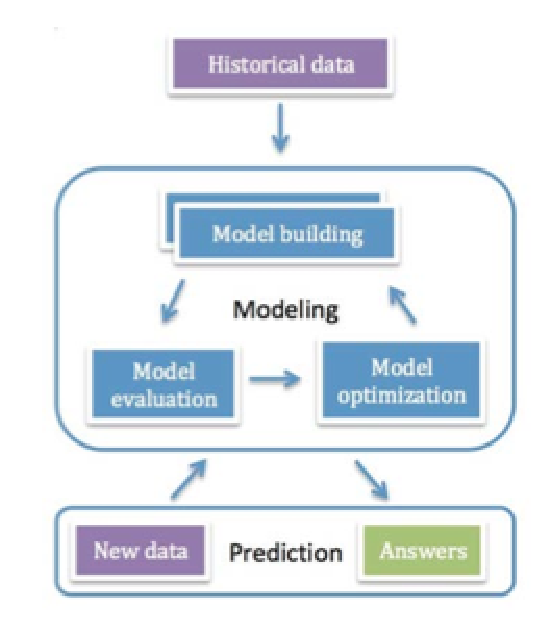
\includegraphics[keepaspectratio=true, scale=0.7]{editaveis/images/mlworkflow.eps}
            \caption{\textit{Workflow} básico de ML.}
            Fonte : Adaptado de \cite{brink2015}
    \end{figure}

\subsection{Tipos de aprendizado}
    \begin{itemize}
        \item Supervisionado: No aprendizado supervisionado, uma massa de dados de treinamento é rodada pelo programa possuindo labels características que as classificam, e no momento em que um novo dado aparece sem essa label (dado de teste), espera-se que o programa seja capaz de predizer qual a classificação do dado.
        \item Não Supervisionado: No aprendizado não supervisionado, a massa de dados de treinamento é a mesma dos dados de teste, pois estes dados não possuem labels que distingüem características. Dessa forma o programa reconhece as características a cada novo dado entregue e começa a fazer a separação de forma autônoma. \cite{chao2011}
        \item Reforço: No aprendizado por reforço, o programa ao receber um sinal de entrada dispara uma ação que muda o valor deste sinal. Assim que o valor do sinal de entrada é alterado e devolvido, mudando assim o estado do ambiente de aprendizagem. A partir disso é recebida uma nova entrada para disparar outra ação que novamente devolverá um valor diferente alterando o estado do ambiente, com a intenç!ao de sempre se aumentar os valores de interação. \cite{kaelbling1996}
    \end{itemize}

\subsection{Seleção de Características}
    Segundo \cite{Yu2005}, seleção de características é o processo de seleção de um subconjuntos de características a partir de um conjunto original e a optmicidade desta seleção é me dida a partir de um critério de avaliação. Um processo de seleção de características é dividido em quatro fases:

    \begin{itemize}
        \item Definição de um subconjunto;
        \item Avaliação do subconjunto;
        \item Aplicação do critério de avaliação;
        \item Validação do resultado.
    \end{itemize}

    A seleção de características é de suma importância para a aplicação de um modelo de aprendizado de máquina, pois é a partir de um bom subconjunto de características que resultados mais precisos são encontrados.

    \subsection{Modelos de Seleção de Características}
        Segundo \cite{Yu2005} os métodos de seleção de características são divididos em três tipos diferentes: modelo de filtro, modelo de envelopamento e o modelo híbrido.

        O modelo de filtro seleciona o subconjunto de características a serem usadas utilizando-se basicamente das próprias características, sem a utilização de um algorítmo de seleção. Isso o torna computacionalmente mais eficiente, principalmente para extração de subconjuntos de características de bases de dados muito extensas.

        O modelo de envelopamento utiliza um algorítmo pré determinado para a seleção do melhor subconjunto de características possível, e para garantir que o subconjunto escolhido seja o melhor possível, o modelo utiliza-se de um classificador próprio que avalia cada subconjunto gerado. Dessa forma o modelo de envelopamento é computacionalmente mais caro e lento conforme o tamamnho do conjunto de dados iniciais aumenta, porém este método garante melhoras resultados.

        O modelo híbrido, combina os modelos de filtro e envelopamento para tentar extrair a melhor característica de cada um. Sendo assim, o modelo híbrido utiliza-se da generalização proposta no modelo de filtro para extrair um primeiro subconjunto, ainda grande de características, para redução do espaço de pesquisa e em seguida aplica o classificador utilizado no modelo de envelopamento para a partir daí conseguir um novo subconjunto menor e otimizado. \cite{Sutha2015}

    \subsection{Método de seleção a ser aplicado}

        O método de seleção a ser aplicado será o \textit{Linear Forward Selection}. Este método utiliza o modelo de seleção de envelopamento e o algorítmo \textit{sequential forward generation} para realizar a busca de características que irão integrar o subconjunto.

        Este metodo funciona ranqueando todas as características, segundo alguma medida pré determinada, e construindo N subconjuntos a partir das características melhores ranqueadas. Por exemplo, a característica A$_1$ foi a melhor ranqueada, seguida por A$_2$ e A$_3$. Neste caso os subconjuntos S$_n$ a serem construídos serão dados da seguinte forma: S$_1$ {A$_1$}, S$_2$ {A$_1$, A$_2$}, S$_3$ {A$_1$, A$_2$, A$_3$} e a ssim por diante conforme a quantidade de características.

        A partir daí, é feita a avaliação de cada subconjunto de acordo com algum classificador, e o subconjunto melhor ranqueado será o escolhido. Este método, por trabalhar a exaustão na busca de subconjuntos apresenta o melhor subconjunto possível, em detrimento de uma eficiência computacional baixa e de um tempo de resposta mais alto em relação a outros métodos.\cite{Franco2015}

\section{Amputações}
    O termo amputação deriva do latim com o significado de “em volta de” e “podar/retirar”, respectivamente, “ambi” e “putatio”, sendo assim pode-se definir amputação como uma retirada cirúrgica ou não, total ou parcial de um membro.  As principais causas de amputações são traumatismo, doenças vasculares periféricas, deficiência congênita, doenças infecciosas e patologias malignas \cite{Carvalho2003}, algumas menos frequentes como esmagamento e queimaduras térmicas e, ou elétricas (FRIEDMANN; 1994). As decisões das amputações devem ser tomadas com calma e precisão, afim do indivíduo ter tempo de amadurecer a respeito das modificações fisiológicas e se adaptarem psicologicamente (DOWNIE,1983).


As referências em relação às amputações possuem dados tão antigos que datam desde 1500 a.C. descritos em manuscrito indiano (\textit{Rig-Veda}) relatando a história da rainha Vishpla que teria tido o membro inferior amputado durante uma batalha (FERNANDES; 2007). Os relatos de amputações feitas de maneira cirúrgicas apenas foram realizadas no início da época pré-cristã, ainda que não houvesse características operatórias, apresentam-se como as primeiras cirurgias de amputação. Porém, não houve nenhum relato citando ou descrevendo as primeiras amputações transtibiais e transfemorias.


Outras evidências de amputações são pinturas em cavernas espanholas e francesas de aproximadamente 38 mil anos, em que apareciam mutilações de membros. Enquanto em um poema escrito em 3500 a.C. que relata a história de uma rainha de guerra, que teve um membro inferior amputado, apresenta a primeira referência de próteses, pois a rainha confeccionou uma prótese de ferro para retornar a guerra. (PEDRINELLI; 2004, CARVALHO; 1999).

A incidência das amputações de membros inferiores no Brasil são de em média 40.000 amputações ao ano, tendo como principais causas complicações da diabetes, e origens traumáticas, sendo que as causas são um dos fatores que influenciam na protetização e cicatrização \cite{Reis2012}.

\subsection{Amputação em membros inferiores}
    Segundo \cite{Barreto2013}, os membros inferiores possuem, via de regra, uma maior chance de serem submetidos à uma cirurgia de amputação em comparação aos membros superiores.

    As amputações de membros inferiores, de forma geral, apresentam níveis de amputação e diferentes observações para realização de processo cirúrgico.  O procedimento cirúrgico e os resíduos biológicos podem facilitar ou dificultar a adaptação do individuo e assim decidir o uso de prótese adequada.

    Os resíduos biológicos, tais como ossos, irão sustentar os tecidos moles. Com isso, deverão ser seccionados de forma que distribuam as cargas para facilitar a protetização, não afetando os tecidos nobres próximos (PEDRINELLI, 2004). As articulações devem ser preservadas desde que sejam favoráveis a uma cicatrização com ausência de infecções parcial ou invasivas, afim de proporcionar uma reabilitação protética adequada e rápida, o que justifica a importância de uma boa avaliação para a prescrição da reabilitação (O‘SULLIVAN; 2005).

    Para a reabilitação protética, devem ser levado em concideração que as amputações transfemorais e transtibiais apresentam peculiaridades e diferentes níveis. No processo cirúrgico, deve-se ter o cuidado para que não haja saliências ou arestas ósseas e a musculatura posterior deve ser rebatida anteriormente para que ocorra formação de coxim (musculatura residual), afim de facilitar a mioplastia (sutura dos músculos e fáscias posteriores na fáscia profunda dos músculos anteriores, ou seja, fixação dos músculos antagonistas aos agonistas) e miodese (reinserção de musculatura ao ponto ósseo), pois tais procedimentos melhoram propriocepção, circulação e controle de coto (CARVALHO; 1999). Além disso, vale ressaltar a importância de identificar e reparar as artérias e veias importantes para vascularização do coto.

    A amputação transfemoral trata-se de uma a retirada do membro com nível de corte entre a desarticulação do joelho e a articulação do quadril, com classificações de longa, média ou curta de acordo com o nível de preservação do comprimento do fêmur. Sendo que as amputações de membros inferiores causam alterações estruturais, mecânicas e metabólicas, sendo essas alterações formas de adaptações a nova condição corporal (SOUSA et al; 2017).

    O coto é de extrema importância para a reabilitação do paciente, dor e desconforto, pois problemas como cicatrizes cutâneas aderentes ou invaginadas, deficiência nos tecidos e pele friável, são os maiores causadores de dor e desconforto. Porém, sabe-se que atualmente existem técnicas para corrigir e evitar tais problemas afim de reduzir as consequências negativas de uma amputação. Tais técnicas como meias em gel, diminuem tais impactos, bem como diminuem a dor e pressão sobre as zonas de impacto e torsão, reduzindo o gasto energético dos mesmos (CARVALHO; 1999, O‘SULLIVAN; 2005).

    Essas alterações a nível de coto residual e seus impactos no processo de reabilitação e protetização necessitam de uma avaliação fisioterapêutica e médica detalhada, para um bom norteamento para a condução do tratamento. Sendo assim, esse trabalho permite a realização de forma automatizada de uma boa avaliação (PRIM et al; 2016).



\chapter[Metodologia]{Metodologia}
    \part{Metodologia}
\chapter[Metodologia]{Metodologia}

Tendo como meta a definição de um modelo de ML para ser aplicada em uma RNA a ser treinada para detecção de intrusão, a estratégia a ser seguida é o conceito de \textit{feature engineering} presente dentro de \textit{machine learning}.

\section{Feature Engineering}
    <aqui vai a aplicação a partir de uma linha retirada do HBase>

\chapter{Resultados Alcançados}
    \part{Resultados}
\chapter[Resultados]{Resultados}

    De acordo com a proposta de \textit{feature engineering} apresentada e utilizando uma amostra de dados de fluxos de rede este capítulo apresentará os resultados atingidos até esta etapa do trabalho.

    \section{Features}
        Como no modelo de dados utilizado para definição das \textit{features} é uma lista de dados retornada por uma consulta em um banco de dados, as \textit{features} definidas para representar um fluxo de dados, que poderá ser definido como malicioso ou não, serão expostas com a mesma nomenclatura do retorno da consulta:
        \\
        \begin{lstlisting}
          column=flow:avg_packet_size;
        \end{lstlisting}

        \begin{lstlisting}
          column=flow:bytes;
        \end{lstlisting}

        \begin{lstlisting}
          column=flow:detected_protocol;
        \end{lstlisting}

        \begin{lstlisting}
          column=flow:packets;
        \end{lstlisting}

        \begin{lstlisting}
          column=event:classification_id;
        \end{lstlisting}

        \begin{lstlisting}
          column=event:priority_id;
        \end{lstlisting}

        \begin{lstlisting}
          column=event:signature_id.
        \end{lstlisting}


        Estas \textit{features} foram escolhidas pois elas definem um fluxo comum, no caso da leitura e aprendizagem de column=flow , e sempre que no mesmo registro a coluna column=event aparecer, para o processo de aprendizado significará que este é um tipo de fluxo que deverá ser marcado como malicioso, e é basicamente definido pelas \textit{features} escolhidas.

        Os próximos passos seguindo o conceito de \textit{feature engineering} seriam o treinamento e avaliação deste modelo, que neste momento ainda não podem ser completos pois esta definição, durante o desenvolvimento deste trabalho, não é somente para ser aplicada nos conceitos de ML, mas para fazer a separação dos dados e treinar uma RNA, que ainda será produzida.